\documentclass[../main.tex]{subfiles}
\begin{document}

% פרק 2: אקוסיסטם הבינה המלאכותית - מפת הכלים למנהל המודרני
% מחברים: דר' יורם סגל ופרופסור ערן שריף
% Compiler: LuaLaTeX

% Set chapter counter for standalone compilation (chapter 2)
\setcounter{chapter}{1}

\chapter{אקוסיסטם הבינה המלאכותית -- מפת הכלים למנהל המודרני}

\section*{מטרות הלמידה}
\begin{itemize}
\item הכרת כל רכיבי האקוסיסטם: מודלי שפה, ספריות, מוטמעים, בסיסי נתונים
\item הבנת היחסים והתלויות בין הרכיבים השונים
\item יכולת לקבל החלטות מושכלות על בחירת טכנולוגיות
\item הערכת עלויות וביצועים של פתרונות שונים
\end{itemize}

\section{פתח דבר: מסע בג'ונגל הטכנולוגי}

דמיינו את עצמכם עומדים בפתחו של יער עצום. מכל עבר צצים שמות זרים: \en{OpenAI}, \en{LangChain}, \en{Pinecone}, \en{ChromaDB}. כל כלי מבטיח פלאים, כל ספק מציע את הפתרון המושלם. עבור מנהל שרוצה להטמיע בינה מלאכותית בארגון שלו, הבחירה הנכונה יכולה להיות מכרעת -- ההבדל בין הצלחה מסחררת לבין כישלון יקר.

בפרק הקודם למדנו מהם מודלי שפה גדולים ומה הכוח שלהם. אבל מודל שפה לבדו, כמו מנוע בלי מכונית, אינו מספיק כדי לנסוע. צריך אקוסיסטם שלם: ספריות שמחברות בין רכיבים, מסדי נתונים שמאחסנים זיכרון, כלים שמנהלים תהליכים אוטומטיים, ופלטפורמות שמאפשרות לכל זה לעבוד יחד בהרמוניה.

הפרק הזה הוא המפה שלכם לג'ונגל הטכנולוגי. נחלק את האקוסיסטם לרכיבים מרכזיים, נבין מה כל אחד עושה, ונלמד מתי להשתמש במה. בסוף הפרק תדעו לתכנן ארכיטקטורה שלמה, להשוות בין ספקים, ולחשב עלויות. זה לא רק ידע טכני -- זה כוח אסטרטגי.

\section{שכבות האקוסיסטם: ארכיטקטורה מלמעלה למטה}

כדי להבין את האקוסיסטם, נחלק אותו לחמש שכבות מרכזיות:

\subsection{שכבת הליבה: מודלי השפה}

זוהי השכבה הבסיסית -- המוח של המערכת. כאן יושבים מודלי השפה הגדולים עצמם. יש לנו שני מסלולים עיקריים:

\textbf{ספקי ענן (\en{Cloud Providers}):} אלו חברות שמריצות מודלים ענקיים על תשתיות ענן ומאפשרות לנו לגשת אליהם דרך \en{API}. המובילים:

\begin{itemize}
\item \textbf{\en{OpenAI}} -- החלוץ והמוביל. \en{GPT-4}, \en{GPT-4 Turbo}, ו-\en{GPT-3.5} הם הסטנדרט התעשייתי. יתרון מרכזי: בשלות, תיעוד עשיר, ואקוסיסטם תומך ענק. חיסרון: עלות גבוהה יחסית, תלות בספק בודד.

\item \textbf{\en{Anthropic}} -- היריבה המתקדמת. מודל \en{Claude 3.5 Sonnet} ו-\en{Claude Opus 4.5} מציעים חלון הקשר ענק (עד 200,000 טוקנים), דיוק גבוה במשימות מורכבות, ודגש על בטיחות. אידיאלי למשימות הדורשות הבנת הקשר עמוקה.

\item \textbf{\en{Google}} -- \en{Gemini Pro} ו-\en{Gemini Ultra} משלבים מולטימודליות מתקדמת (טקסט, תמונה, וידאו). יתרון משמעותי: אינטגרציה חלקה עם \en{Google Workspace}.

\item \textbf{\en{Meta}} -- \en{Llama 3} (בגרסאות 8B, 70B, 405B) הוא מודל קוד פתוח. למה זה משמעותי? תוכלו להוריד ולהריץ אותו על השרתים שלכם. אין תלות בספק חיצוני, אין דליפת מידע רגיש החוצה.

\item \textbf{\en{DeepSeek}} -- השחקן הסיני המפתיע. \en{DeepSeek-V3} מציע ביצועים מרשימים במחיר נמוך משמעותית. בעיקר למשימות טכניות וקוד.
\end{itemize}

\textbf{מודלים מקומיים (\en{Self-Hosted}):} כאן אנחנו מורידים את המודל ומריצים אותו על החומרה שלנו:

\begin{itemize}
\item \textbf{\en{Llama 3.1 (8B/70B)}} -- מודל קוד פתוח מצוין לריצה מקומית. גרסת 8B רצה אפילו על לפטופ חזק, 70B דורש שרת עם GPU.

\item \textbf{\en{Mistral 7B}} -- קטן, מהיר, יעיל. מצוין לסטארטאפים שרוצים פתרון זול ומקומי.

\item \textbf{\en{Qwen 2.5}} -- מודל סיני מתקדם, מצוין לתמיכה רב-לשונית.
\end{itemize}

למה לבחור ב-\en{Self-Hosted}? שלוש סיבות עיקריות:
\begin{enumerate}
\item \textbf{פרטיות מוחלטת} -- נתונים רגישים לא עוזבים את הארגון.
\item \textbf{עלות צפויה} -- שילמתם על החומרה פעם אחת, אין הפתעות בחשבון.
\item \textbf{התאמה אישית} -- אפשר לעשות \en{Fine-tuning} ייעודי.
\end{enumerate}

\subsection{שכבת החיבור: \en{OpenRouter} -- הרכזת של מודלים}

\en{OpenRouter} הוא כמו שדה תעופה שמחבר אתכם לכל היעדים. במקום לפתוח חשבון בנפרד אצל \en{OpenAI}, \en{Anthropic}, ו-\en{Google}, אתם נרשמים פעם אחת ל-\en{OpenRouter} ומקבלים גישה למעל 100 מודלים שונים דרך \en{API} אחיד.

\textbf{יתרונות מנהליים:}
\begin{itemize}
\item גמישות -- החלפת מודל זה שורת קוד אחת
\item השוואת עלויות -- תוכלו לנסות מודלים שונים בלי להתחייב
\item גיבוי אוטומטי -- אם ספק אחד נופל, \en{OpenRouter} מעביר למודל חלופי
\end{itemize}

\textbf{דוגמה מעשית:} חברת תמיכה טכנית השתמשה ב-\en{GPT-4} לניתוח פניות מורכבות. אבל \en{70\%} מהפניות היו פשוטות, ו-\en{GPT-4} יקר מדי בשבילן. עם \en{OpenRouter} הם יישמו לוגיקה: פניות פשוטות ל-\en{GPT-3.5} (זול), פניות מורכבות ל-\en{Claude Sonnet} (מדויק). חיסכו \en{60\%} בעלויות בלי לוותר על איכות.

\subsection{שכבת הפיתוח: ספריות אינטגרציה}

כדי לבנות מערכת אמיתית, לא מספיק לשלוח בקשה ל-\en{API} ולקבל תשובה. צריך לנהל שיחות, לזכור הקשר, לחבר בסיסי נתונים, לטפל בשגיאות. כאן נכנסות הספריות:

\subsubsection{\en{LangChain} -- הסוכן המקצועי}

\en{LangChain} היא הספרייה הפופולרית ביותר לבניית אפליקציות \en{LLM}. היא מציעה:

\begin{itemize}
\item \textbf{\en{Chains}} -- שרשור פעולות. לדוגמה: קח שאלה $\rightarrow$ חפש במסד נתונים $\rightarrow$ שלח ל-\en{LLM} $\rightarrow$ עצב תשובה.

\item \textbf{\en{Agents}} -- סוכנים אוטונומיים שיודעים לבחור כלים. "איזה טיסות זולות לברלין?" $\rightarrow$ הסוכן מבין שצריך לקרוא ל-\en{API} של טיסות, מנתח תוצאות, ומחזיר תשובה.

\item \textbf{\en{Memory}} -- זיכרון שיחה. ה-\en{LLM} זוכר מה דיברתם לפני \en{10} הודעות.

\item \textbf{\en{Retrievers}} -- חיבור לבסיסי נתונים וקטוריים (נדבר עליהם בהמשך).
\end{itemize}

\textbf{מתי להשתמש ב-\en{LangChain}?} כשאתם בונים משהו מורכב -- סוכן שירות, מערכת \en{RAG}, אוטומציה רב-שלבית.

\subsubsection{\en{LangGraph} -- תזמור תהליכים}

\en{LangGraph} הוא ההמשך של \en{LangChain}, ממוקד בניהול תהליכים מורכבים עם מעברים ותנאים.

דמיינו תהליך אישור הזמנה:
\begin{enumerate}
\item בדיקת מלאי
\item אישור מנהל (אם מעל \en{10,000} ש"ח)
\item שליחה ללוגיסטיקה
\item עדכון לקוח
\end{enumerate}

\en{LangGraph} מאפשר לכם לתכנן את התהליך כגרף זרימה, עם צמתים (פעולות) וקשתות (תנאים). כל צומת יכול להיות \en{LLM}, שאילתת מסד נתונים, או קריאה חיצונית.

\subsubsection{\en{Pydantic AI} -- המובנה והמסודר}

אם \en{LangChain} הוא הסוכן הגמיש, \en{Pydantic AI} הוא הבנקאי המדויק. הספרייה מתמחה במבנה ובולידציה:

\begin{itemize}
\item הגדרת מבני נתונים נוקשים
\item ולידציה אוטומטית של תשובות \en{LLM}
\item אכיפת פורמטים (\en{JSON Schema})
\end{itemize}

\textbf{דוגמה:} אתם רוצים ש-\en{LLM} יחלץ מפניית לקוח: שם, מייל, נושא, רמת דחיפות. \en{Pydantic AI} מגדיר מבנה קפדני, ואם ה-\en{LLM} מחזיר משהו שלא תואם -- יש שגיאה מיידית.

\subsection{שכבת ההטמעה: \en{Embeddings} ומסדי נתונים וקטוריים}

אחת התובנות המרכזיות בעולם ה-\en{AI} המודרני היא שמילים הן לא רק תווים -- יש להן משמעות גיאומטרית. טכנולוגיית \en{Embeddings} הופכת טקסט למספרים (וקטורים), כך שמחשב יכול "להבין" דמיון סמנטי.

\subsubsection{מהם \en{Embeddings}?}

תארו לעצמכם מרחב של מאות או אלפי ממדים. כל מילה או משפט הוא נקודה במרחב הזה. משפטים דומים במשמעות קרובים גיאומטרית; משפטים שונים רחוקים.

לדוגמה:
\begin{itemize}
\item \en{"} כלב\en{"} ו-\en{"}גור\en{"} -- קרובים מאוד
\item \en{"}כלב\en{"} ו-\en{"}מכונית\en{"} -- רחוקים
\end{itemize}

\textbf{למה זה חשוב?} כי ככה בונים חיפוש סמנטי. במקום לחפש מילת מפתח מדויקת (כמו \en{Google} פעם), אפשר לחפש לפי כוונה.

\textbf{שאלה:} "איך מגישים תביעת ביטוח?"
\textbf{מסמך במערכת:} "הליך הגשת דרישה לפיצוי"

חיפוש רגיל לא ימצא את זה -- אין מילים משותפות. חיפוש וקטורי כן.

\subsubsection{מודלי \en{Embedding} מובילים}

\begin{itemize}
\item \textbf{\en{OpenAI Text-Embedding-3}} -- הסטנדרט. קל לשימוש, איכות מצוינת. גרסת \en{small} (זולה) וגרסת \en{large} (מדויקת).

\item \textbf{\en{NV-Embed-v2}} -- מודל מתקדם מבית \en{NVIDIA}. מצוין לטקסטים טכניים ומדעיים.

\item \textbf{\en{BGE-M3}} -- מודל סיני רב-לשוני. תומך במעל 100 שפות, כולל עברית. קוד פתוח.
\end{itemize}

\subsubsection{מסדי נתונים וקטוריים}

אחרי שהפכנו טקסט לוקטורים, איפה נאחסן אותם? מסד נתונים רגיל (\en{MySQL}, \en{PostgreSQL}) לא יודע לעבוד עם חיפוש וקטורי. צריך מסד נתונים וקטורי (\en{Vector Database}).

\textbf{\en{Pinecone} -- הענן המנוהל:}
\begin{itemize}
\item \textbf{יתרונות:} לא צריך להתקין כלום. שירות ענן מנוהל, סקיילבילי, מהיר.
\item \textbf{חסרונות:} עלות חודשית, תלות בספק.
\item \textbf{מתי להשתמש:} כשאתם רוצים לעלות מהר, בלי להתעסק בתשתיות.
\end{itemize}

\textbf{\en{Chroma} -- הפתרון המקומי:}
\begin{itemize}
\item \textbf{יתרונות:} קוד פתוח, חינמי, רץ על השרת שלכם.
\item \textbf{חסרונות:} אתם צריכים לנהל: גיבויים, ביצועים, סקייל.
\item \textbf{מתי להשתמש:} כשאתם בשלב \en{POC}, או כשאתם רוצים שליטה מלאה.
\end{itemize}

\textbf{\en{Weaviate} -- הכלי ההיברידי:}
\begin{itemize}
\item \textbf{יתרונות:} תומך גם בחיפוש וקטורי וגם בחיפוש טקסט רגיל. אינטגרציות עשירות.
\item \textbf{חסרונות:} מורכב יותר להקמה.
\item \textbf{מתי להשתמש:} כשאתם צריכים גמישות מקסימלית.
\end{itemize}

\textbf{\en{Qdrant} -- המהיר:}
\begin{itemize}
\item \textbf{יתרונות:} ביצועים מצוינים, נכתב ב-\en{Rust} (מהיר ויעיל).
\item \textbf{חסרונות:} קהילה קטנה יותר.
\item \textbf{מתי להשתמש:} כשמהירות היא קריטית.
\end{itemize}

\subsection{שכבת האוטומציה: כלים אגנטיים}

השכבה העליונה היא שכבת התזמור -- הכלים שגורמים לכל המערכת לעבוד יחד ולהריץ תהליכים אוטומטיים.

\subsubsection{\en{LangGraph} (שוב, אבל בהקשר אחר)}

כבר דיברנו עליו כספרייה, אבל הוא גם כלי תזמור. \en{LangGraph} מאפשר לכם לבנות תהליכים רב-שלביים שבהם סוכנים שונים מתקשרים זה עם זה, מעבירים מידע, ומקבלים החלטות.

\subsubsection{\en{AutoGen} -- צוותי סוכנים}

\en{AutoGen} (מבית \en{Microsoft}) הוא פריימוורק לבניית מערכות רב-סוכן. דמיינו שאתם בונים מערכת לניהול פרויקטים:

\begin{itemize}
\item \textbf{סוכן תכנון} -- מנתח דרישות ובונה תוכנית עבודה
\item \textbf{סוכן ביצוע} -- מקצה משימות לאנשי צוות
\item \textbf{סוכן בקרה} -- עוקב אחרי התקדמות ומתריע על עיכובים
\end{itemize}

כל סוכן הוא \en{LLM} עם הנחיות (\en{System Prompt}) ייעודיות. \en{AutoGen} מנהל את התקשורת ביניהם.

\subsubsection{\en{n8n} -- אוטומציה חזותית}

\en{n8n} הוא כלי \en{No-Code / Low-Code} לאוטומציה. במקום לכתוב קוד, אתם גוררים בלוקים ומחברים אותם.

\textbf{דוגמה:}
\begin{enumerate}
\item כל פניית לקוח במייל $\rightarrow$
\item \en{LLM} מנתח ומקטלג $\rightarrow$
\item אם דחוף: שולח SMS למנהל $\rightarrow$
\item אם רגיל: פותח כרטיס ב-\en{Jira}
\end{enumerate}

הכל בלי לכתוב שורת קוד אחת.

\subsubsection{\en{Zapier} -- השחקן הוותיק}

\en{Zapier} קיים הרבה לפני \en{AI}, אבל הוא השתלב מצוין. תומך באלפי אינטגרציות (Gmail, Slack, Salesforce, Notion...). לאחרונה הוסיף תמיכה ב-\en{OpenAI} ו-\en{Anthropic}.

\textbf{מתי \en{n8n} ומתי \en{Zapier}?}
\begin{itemize}
\item \en{Zapier} -- אם אתם רוצים פשטות ותמיכה ענקית בשירותים חיצוניים
\item \en{n8n} -- אם אתם רוצים שליטה, תמחור טוב יותר, ואפשרות ל-\en{Self-Hosted}
\end{itemize}

\section{מתי להשתמש במה: מטריצת החלטות}

עכשיו שאנחנו מכירים את כל השחקנים, איך בוחרים? הנה מטריצה מנהלית:

\subsection{בחירת ספק \en{LLM}}

\begin{hebrewtable}[h]
\caption{מטריצת בחירת מודל שפה}
\begin{rtltabular}{|m{4cm}|m{4cm}|m{3.5cm}|}
\hline
\rowcolor{blue!15}
\textbf{\hebheader{הסבר}} & \textbf{\hebheader{בחירה}} & \textbf{\hebheader{קריטריון}} \\
\hline
\hebcell{הטובים ביותר לחשיבה מורכבת} & \encell{\en{Claude Opus} / \en{GPT-4}} & \hebcell{דיוק גבוה, משימות מורכבות} \\
\hline
\hebcell{יחס מחיר-ביצועים מעולה} & \encell{\en{GPT-3.5} / \en{DeepSeek}} & \hebcell{עלות נמוכה, נפח גבוה} \\
\hline
\hebcell{שום דבר לא עוזב את הארגון} & \encell{\en{Llama 3 (Self-Hosted)}} & \hebcell{פרטיות, נתונים רגישים} \\
\hline
\hebcell{תמיכה בתמונות ווידאו} & \encell{\en{Gemini Pro} / \en{GPT-4 Vision}} & \hebcell{מולטימודליות} \\
\hline
\hebcell{עד \en{200K} טוקנים} & \encell{\en{Claude 3.5 Sonnet}} & \hebcell{חלון הקשר ענק} \\
\hline
\end{rtltabular}
\end{hebrewtable}

\subsection{בחירת מסד נתונים וקטורי}

\begin{hebrewtable}[h]
\caption{מטריצת בחירת מסד נתונים וקטורי}
% RTL ORDER: rightmost column first, leftmost column last
% Use m{} columns for vertical centering
\begin{rtltabular}{|m{4cm}|m{4cm}|m{3.5cm}|}
\hline
\rowcolor{blue!15}
\textbf{\hebheader{הסבר}} & \textbf{\hebheader{בחירה}} & \textbf{\hebheader{תרחיש}} \\
\hline
\hebcell{חינמי, פשוט, מקומי} & \encell{\en{Chroma}} & \hebcell{\en{POC} / אב טיפוס} \\
\hline
\hebcell{מנוהל, אמין, לא צריך \en{DevOps}} & \encell{\en{Pinecone}} & \hebcell{ייצור, סטארטאפ} \\
\hline
\hebcell{שליטה מלאה, גמישות} & \encell{\en{Weaviate} או \en{Qdrant}} & \hebcell{ארגון גדול, \en{On-Prem}} \\
\hline
\hebcell{אופטימיזציה קיצונית} & \encell{\en{Qdrant}} & \hebcell{צורך במהירות מקסימלית} \\
\hline
\end{rtltabular}
\end{hebrewtable}

\subsection{החלטת ענן מול \en{On-Premise}}

\begin{figure}[h]
\centering
\begin{english}
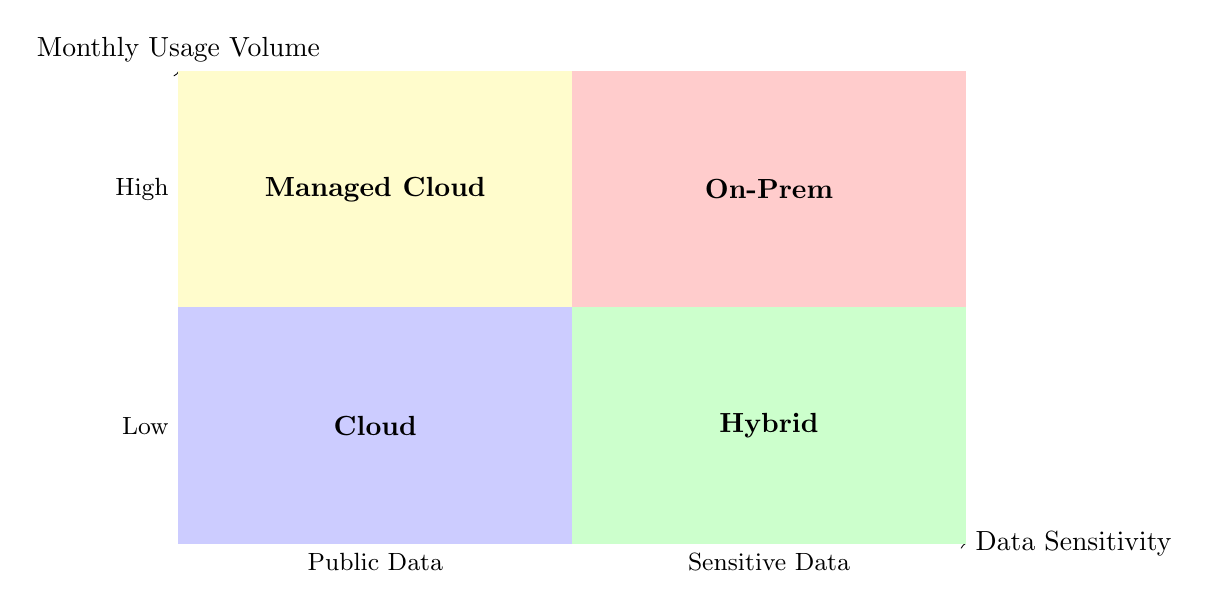
\begin{tikzpicture}
% X-axis: Data Sensitivity
% Y-axis: Monthly Usage Volume
\draw[->] (0,0) -- (10,0) node[right] {Data Sensitivity};
\draw[->] (0,0) -- (0,6) node[above] {Monthly Usage Volume};

% Regions
\fill[blue!20] (0,0) rectangle (5,3);
\node at (2.5,1.5) {\textbf{Cloud}};

\fill[green!20] (5,0) rectangle (10,3);
\node at (7.5,1.5) {\textbf{Hybrid}};

\fill[red!20] (5,3) rectangle (10,6);
\node at (7.5,4.5) {\textbf{On-Prem}};

\fill[yellow!20] (0,3) rectangle (5,6);
\node at (2.5,4.5) {\textbf{Managed Cloud}};

% Labels
\node[below] at (2.5,0) {\small Public Data};
\node[below] at (7.5,0) {\small Sensitive Data};
\node[left] at (0,1.5) {\small Low};
\node[left] at (0,4.5) {\small High};
\end{tikzpicture}
\end{english}
\caption{מטריצת החלטה: ענן מול \en{On-Premise}}
\end{figure}

\textbf{פענוח המטריצה:}
\begin{itemize}
\item \textbf{רביע שמאלי תחתון (כחול):} נתונים לא רגישים, נפח נמוך $\rightarrow$ \en{Cloud} (\en{OpenAI}, \en{Anthropic})
\item \textbf{רביע ימני תחתון (ירוק):} נתונים רגישים, נפח נמוך $\rightarrow$ \en{Hybrid} (חלק בענן, חלק מקומי)
\item \textbf{רביע ימני עליון (אדום):} נתונים רגישים, נפח גבוה $\rightarrow$ \en{On-Prem} (\en{Llama 3} על שרתים פנימיים)
\item \textbf{רביע שמאלי עליון (צהוב):} נתונים לא רגישים, נפח גבוה $\rightarrow$ \en{Cloud} מנוהל עם הסכם ארגוני
\end{itemize}

\section{נוסחאות מנהליות: חשבון כלכלי}

כמנהלים, אנחנו צריכים להצדיק כל החלטה טכנולוגית בשפה כלכלית. הנה שתי נוסחאות קריטיות:

\subsection{נוסחת \en{TCO} -- עלות בעלות כוללת}

\begin{equation}
\text{TCO} = C_{\text{license}} + C_{\text{infra}} + (C_{\text{HR}} \times 12)
\end{equation}

\textbf{פירוק הנוסחה:}
\begin{itemize}
\item $C_{\text{license}}$ -- עלות רישוי שנתית (מנויים ל-API, רישיונות תוכנה)
\item $C_{\text{infra}}$ -- עלות תשתיות (שרתים, אחסון, רשת, חשמל)
\item $C_{\text{HR}}$ -- עלות כוח אדם חודשית (מפתחים, \en{DevOps}, מנהלי מערכת)
\end{itemize}

\textbf{דוגמה \en{1}: פתרון ענן טהור (\en{OpenAI})}
\begin{itemize}
\item רישוי: \en{\$5,000} לחודש (\en{\$60,000} לשנה)
\item תשתיות: \en{\$0} (ספק מנוהל)
\item כוח אדם: מפתח חצי משרה (\en{\$4,000} לחודש)
\end{itemize}

\begin{equation}
\text{TCO} = 60{,}000 + 0 + (4{,}000 \times 12) = \$108{,}000
\end{equation}

\textbf{דוגמה \en{2}: פתרון \en{On-Premise} (\en{Llama 3})}
\begin{itemize}
\item רישוי: \en{\$0} (קוד פתוח)
\item תשתיות: שרת עם \en{8 GPUs} (\en{\$80,000} לשנה, פחת על \en{5} שנים = \en{\$16,000} לשנה) + חשמל וקירור (\en{\$12,000} לשנה)
\item כוח אדם: מפתח + \en{DevOps} (\en{\$10,000} לחודש)
\end{itemize}

\begin{equation}
\text{TCO} = 0 + 28{,}000 + (10{,}000 \times 12) = \$148{,}000
\end{equation}

\textbf{מסקנה:} בטווח הקצר, הענן זול יותר. אבל אם נפח השימוש גדל -- \en{On-Prem} משתלם יותר.

\subsection{נוסחת \en{Latency} -- זמן תגובה}

\begin{equation}
T_{\text{total}} = T_{\text{network}} + T_{\text{processing}} + T_{\text{model}}
\end{equation}

\textbf{פירוק הנוסחה:}
\begin{itemize}
\item $T_{\text{network}}$ -- זמן העברת הבקשה והתשובה ברשת (RTT)
\item $T_{\text{processing}}$ -- זמן עיבוד מקדים (Embedding, חיפוש במסד נתונים)
\item $T_{\text{model}}$ -- זמן ההסקה של המודל עצמו
\end{itemize}

\textbf{דוגמה: שאילתת \en{RAG}}
\begin{itemize}
\item $T_{\text{network}}$ = \en{50ms} (לענן בחו"ל) או \en{2ms} (לשרת מקומי)
\item $T_{\text{processing}}$ = \en{100ms} (\en{Embedding} + חיפוש ב-\en{Pinecone})
\item $T_{\text{model}}$ = \en{800ms} (\en{GPT-4})
\end{itemize}

\textbf{סה"כ (ענן):}
\begin{equation}
T_{\text{total}} = 50 + 100 + 800 = 950 \text{ms}
\end{equation}

\textbf{סה"כ (מקומי):}
\begin{equation}
T_{\text{total}} = 2 + 100 + 800 = 902 \text{ms}
\end{equation}

\textbf{מסקנה:} זמן רשת נראה קטן, אבל בנפח גבוה (אלפי בקשות ביום) -- הוא משמעותי.

\section{השוואת מחירים: מי הכי משתלם?}

מחירי \en{API} משתנים כל הזמן, אבל הנה תמונת מצב (נכונה לדצמבר 2024):

\begin{hebrewtable}[h]
\caption{השוואת מחירי מודלים מרכזיים}
% RTL ORDER: rightmost column first, leftmost column last
% Use m{} columns for vertical centering
\small
\begin{rtltabular}{|m{2cm}|m{2.5cm}|m{2.5cm}|m{3cm}|}
\hline
\rowcolor{blue!15}
\textbf{\hebheader{משוקלל*}} & \textbf{\hebheader{פלט (\$/1M טוקנים)}} & \textbf{\hebheader{קלט (\$/1M טוקנים)}} & \textbf{\hebheader{מודל}} \\
\hline
\encell{\$20.00} & \encell{\$30.00} & \encell{\$10.00} & \encell{GPT-4 Turbo} \\
\hline
\encell{\$1.00} & \encell{\$1.50} & \encell{\$0.50} & \encell{GPT-3.5 Turbo} \\
\hline
\encell{\$9.00} & \encell{\$15.00} & \encell{\$3.00} & \encell{Claude 3.5 Sonnet} \\
\hline
\encell{\$0.75} & \encell{\$1.25} & \encell{\$0.25} & \encell{Claude 3 Haiku} \\
\hline
\encell{\$1.00} & \encell{\$1.50} & \encell{\$0.50} & \encell{Gemini Pro} \\
\hline
\encell{\$0.69} & \encell{\$1.10} & \encell{\$0.27} & \encell{DeepSeek-V3} \\
\hline
\encell{\$0.00***} & \encell{\$0.00} & \encell{\$0.00} & \encell{Llama 3.1 70B**} \\
\hline
\end{rtltabular}
\begin{flushleft}
\small
* משוקלל: הנחה של \en{50\%} קלט, \en{50\%} פלט\\
** דרך \en{OpenRouter} או ספקים אחרים\\
*** עלות אפסית לשימוש, אבל יש עלות תשתית
\end{flushleft}
\end{hebrewtable}

\textbf{תובנות מהטבלה:}
\begin{enumerate}
\item \en{GPT-4} הוא הכי יקר -- פי \en{20} מ-\en{GPT-3.5}. האם התוצאה מצדיקה? תלוי במשימה.
\item \en{Claude Haiku} ו-\en{DeepSeek} -- אלטרנטיבות זולות ומצוינות לנפח גבוה.
\item \en{Llama 3} -- עלות אפסית לשימוש, אבל צריך להשקיע בתשתית.
\end{enumerate}

\section{דוגמאות מעשיות מהשטח}

\subsection{דוגמה 1: סטארטאפ בשלב \en{Seed} -- בחירת \en{Stack}}

\textbf{תרחיש:} חברת \en{FinTech} עם \en{5} עובדים, רוצה לבנות עוזר פיננסי אישי. תקציב: \en{\$2,000} לחודש.

\textbf{צרכים:}
\begin{itemize}
\item עיבוד שאלות פיננסיות פשוטות (\en{80\%}) ומורכבות (\en{20\%})
\item אחסון ידע על מוצרים פיננסיים (\en{200} מסמכים)
\item אינטגרציה עם בנקים (\en{API})
\end{itemize}

\textbf{ארכיטקטורה מומלצת:}
\begin{itemize}
\item \textbf{\en{LLM}:} \en{OpenRouter} עם \en{GPT-3.5} לשאלות פשוטות, \en{Claude Sonnet} למורכבות
\item \textbf{\en{Embeddings}:} \en{OpenAI Text-Embedding-3-small} (זול)
\item \textbf{\en{Vector DB}:} \en{Pinecone} תוכנית חינמית (עד \en{100K} וקטורים)
\item \textbf{\en{Framework}:} \en{LangChain} (קהילה גדולה, הרבה דוגמאות)
\item \textbf{\en{Automation}:} \en{n8n} (\en{Self-Hosted}, חינמי)
\end{itemize}

\textbf{עלויות:}
\begin{itemize}
\item \en{OpenRouter}: \en{\$800}/חודש (בממוצע)
\item \en{Pinecone}: \en{\$0} (תוכנית חינמית)
\item \en{n8n}: \en{\$0} (\en{Self-Hosted} על \en{AWS EC2} קטן, \en{\$20}/חודש)
\item פיתוח: מפתח אחד חצי משרה
\end{itemize}

\textbf{סה"כ: \en{\$820}/חודש} -- מתחת לתקציב, עם מרווח לגדילה.

\subsection{דוגמה 2: ארגון גדול -- מעבר מ-\en{ChatGPT} לפתרון ארגוני}

\textbf{תרחיש:} חברת ייעוץ עם \en{500} עובדים. כרגע כולם משתמשים ב-\en{ChatGPT} אישי. הבעיה: אין שליטה, נתונים דולפים, אין התאמה אישית.

\textbf{דרישות:}
\begin{itemize}
\item גישה למידע פנימי (מדיניות, פרויקטים, לקוחות)
\item פרטיות מלאה -- נתונים לא יוצאים
\item יכולת ביקורת -- מי שאל מה ומתי
\item התאמה אישית לתהליכים של הארגון
\end{itemize}

\textbf{ארכיטקטורה מומלצת:}
\begin{itemize}
\item \textbf{\en{LLM}:} \en{Azure OpenAI} (גרסה ארגונית -- נתונים לא משמשים לאימון)
\item \textbf{\en{RAG}:} \en{Weaviate} על שרתים פנימיים
\item \textbf{\en{Embeddings}:} \en{Azure OpenAI Embeddings}
\item \textbf{\en{Framework}:} \en{LangChain} עם \en{LangSmith} (ניטור ולוגים)
\item \textbf{\en{UI}:} פורטל פנימי מבוסס \en{Streamlit}
\end{itemize}

\textbf{יתרונות:}
\begin{itemize}
\item נתונים נשארים ב-\en{Tenant} הארגוני של \en{Azure}
\item אפשר לחבר לכל מסדי הנתונים הפנימיים
\item לוגים מלאים לביקורת
\item התאמה אישית -- אפשר לכוון את המודל לתהליכים ספציפיים
\end{itemize}

\textbf{עלויות (הערכה):}
\begin{itemize}
\item \en{Azure OpenAI}: \en{\$15,000}/חודש (\en{500} משתמשים)
\item \en{Weaviate} על \en{Azure VM}: \en{\$2,000}/חודש
\item פיתוח ותחזוקה: \en{2} מפתחים (\en{\$20,000}/חודש)
\end{itemize}

\textbf{סה"כ: \en{\$37,000}/חודש} -- נשמע יקר? לא בהשוואה ל-\en{500} רישיונות \en{ChatGPT Plus} (\en{\$10,000}\allowbreak/חודש) ללא שליטה וללא התאמה אישית.

\subsection{דוגמה 3: החלטת \en{Build vs Buy}}

\textbf{תרחיש:} חברת \en{e-commerce} רוצה סוכן שירות אוטומטי. השאלה: לקנות פתרון מוכן (כמו \en{Intercom}) או לבנות בעצמנו?

\textbf{ניתוח \en{Build}:}
\begin{itemize}
\item \textbf{עלות פיתוח:} \en{3} חודשי עבודה של מפתח (\en{\$30,000})
\item \textbf{עלות ריצה:} \en{API} + שרתים (\en{\$1,500}/חודש)
\item \textbf{תחזוקה:} רבע משרה (\en{\$3,000}/חודש)
\item \textbf{סה"כ שנה ראשונה:} \en{\$30,000 + (\$4,500 $\times$ 12) = \$84,000}
\end{itemize}

\textbf{ניתוח \en{Buy} (\en{Intercom}):}
\begin{itemize}
\item \textbf{רישוי:} \en{\$5,000}/חודש (\en{500} שיחות ביום)
\item \textbf{אינטגרציה:} חודש עבודה (\en{\$10,000})
\item \textbf{תחזוקה:} כמעט אפסית
\item \textbf{סה"כ שנה ראשונה:} \en{\$10,000 + (\$5,000 $\times$ 12) = \$70,000}
\end{itemize}

\textbf{החלטה:} בשנה הראשונה, \en{Buy} זול יותר. אבל:
\begin{itemize}
\item אם הנפח גדל (\en{1,000} שיחות ביום) -- \en{Intercom} יעלה ל-\en{\$10,000}/חודש
\item פתרון \en{Build} נשאר באותה עלות (או עולה מעט)
\item פתרון \en{Build} מאפשר התאמה מלאה לתהליכים
\end{itemize}

\textbf{המלצה:} התחילו עם \en{Buy} (מהיר, מוכח). אחרי שנה, אם הנפח גדל -- עברו ל-\en{Build}.

\section{תרגילים}

\subsection{תרגיל 1 (תיאורטי): בניית ארכיטקטורה לפרויקט \en{AI}}

\textbf{תרחיש:} אתם סמנכ"ל טכנולוגיות בחברת ביטוח בינונית (\en{200} עובדים). מנכ"ל מבקש מכם לבנות מערכת \en{AI} שתענה על שאלות סוכני הביטוח על מדיניות ותקנות (\en{5,000} מסמכים פנימיים).

\textbf{דרישות:}
\begin{itemize}
\item פרטיות מלאה -- מסמכים רגישים
\item זמן תגובה: עד \en{3} שניות
\item תקציב: \en{\$10,000}/חודש
\item \en{50} שאלות ביום בממוצע
\end{itemize}

\textbf{משימה:}
\begin{enumerate}
\item בחרו ספק \en{LLM} (ענן / מקומי / היברידי)
\item בחרו מודל \en{Embedding}
\item בחרו מסד נתונים וקטורי
\item בחרו ספריית אינטגרציה
\item הצדיקו כל בחירה
\item חשבו \en{TCO} לשנה
\end{enumerate}

\subsection{תרגיל 2 (תיאורטי): חישוב \en{TCO} לשלושה תרחישים}

השוו \en{TCO} לשלוש אפשרויות:

\textbf{תרחיש א': ענן טהור}
\begin{itemize}
\item \en{GPT-4} דרך \en{OpenAI}
\item \en{Pinecone} מנוהל
\item מפתח חצי משרה
\end{itemize}

\textbf{תרחיש ב': היברידי}
\begin{itemize}
\item \en{Azure OpenAI} (ארגוני)
\item \en{Weaviate} על \en{Azure VM}
\item מפתח + מנהל מערכת (שני חצאי משרה)
\end{itemize}

\textbf{תרחיש ג': \en{On-Premise} מלא}
\begin{itemize}
\item \en{Llama 3.1 70B} על שרת פנימי
\item \en{Chroma} מקומי
\item מפתח + \en{DevOps} + מנהל מערכת
\end{itemize}

חשבו \en{TCO} לשנה לכל תרחיש. איזה משתלם לנפח של:
\begin{itemize}
\item \en{1,000} שאלות ביום?
\item \en{10,000} שאלות ביום?
\item \en{100,000} שאלות ביום?
\end{itemize}

\subsection{תרגיל 3 (תיאורטי): ניתוח \en{Trade-offs} בין \en{Pinecone} ל-\en{Chroma}}

מנהל פיתוח שואל אתכם: "למה לא פשוט להשתמש ב-\en{Chroma}? זה בחינם!"

\textbf{משימה:}
\begin{enumerate}
\item רשמו \en{5} יתרונות של \en{Pinecone}
\item רשמו \en{5} יתרונות של \en{Chroma}
\item בנו טבלת החלטה: באיזה מקרים כל אחד עדיף
\item הסבירו למה \en{"}בחינם\en{"} לא תמיד זול יותר
\end{enumerate}

\subsection{תרגיל 4 (תיאורטי): תכנון אסטרטגיית \en{Vendor}}

אתם אחראים על אסטרטגיית \en{AI} ארוכת טווח. מנכ"ל דואג מ-\en{Vendor Lock-in}.

\textbf{משימה:}
\begin{enumerate}
\item הסבירו מהם הסיכונים של תלות בספק בודד
\item תכננו אסטרטגיית \en{Multi-Vendor} (יותר מספק אחד)
\item רשמו \en{3} טכניקות למניעת \en{Lock-in}
\item נתחו: האם \en{OpenRouter} פותר את הבעיה? למה כן \en{/} למה לא?
\end{enumerate}

\subsection{תרגיל 5 (תיאורטי): בניית \en{RFP} לבחירת ספק \en{AI}}

\textbf{תרחיש:} הארגון שלכם רוצה לבחור ספק \en{AI} לטווח ארוך. עליכם לכתוב \en{RFP} (Request for Proposal).

\textbf{משימה:} כתבו \en{RFP} שכולל:
\begin{enumerate}
\item רקע על הארגון וצרכיו
\item דרישות פונקציונליות (מה המערכת צריכה לעשות)
\item דרישות לא-פונקציונליות (ביצועים, אבטחה, זמינות)
\item קריטריוני הערכה (איך תבחרו בין הצעות)
\item לוח זמנים
\end{enumerate}

\subsection{תרגיל 6 (קוד \en{Python}): השוואת מחירי \en{API} בין ספקים}

כתבו סקריפט \en{Python} שמקבל:
\begin{itemize}
\item מספר טוקנים קלט
\item מספר טוקנים פלט
\item מספר בקשות לחודש
\end{itemize}

ומחשב עלות חודשית עבור:
\begin{itemize}
\item \en{GPT-4 Turbo}
\item \en{GPT-3.5 Turbo}
\item \en{Claude 3.5 Sonnet}
\item \en{Gemini Pro}
\end{itemize}

\textbf{בונוס:} הציגו את התוצאות בגרף עמודות.

\textbf{קוד התחלתי:}

\begin{english}
\begin{pythonbox*}[\hebtitle{השוואת מחירי API}]
# API price comparison between providers

# Prices ($/1M tokens) - update with actual prices
PRICING = {
    "GPT-4 Turbo": {"input": 10.0, "output": 30.0},
    "GPT-3.5 Turbo": {"input": 0.5, "output": 1.5},
    "Claude 3.5 Sonnet": {"input": 3.0, "output": 15.0},
    "Gemini Pro": {"input": 0.5, "output": 1.5},
}

def calculate_monthly_cost(model_name, input_tokens,
                          output_tokens, requests_per_month):
    """
    Calculate monthly cost for a given model

    Args:
        model_name: Model name
        input_tokens: Input tokens per request
        output_tokens: Output tokens per request
        requests_per_month: Requests per month

    Returns:
        Monthly cost in dollars
    """
    pricing = PRICING[model_name]

    # Calculate total tokens per month
    total_input = input_tokens * requests_per_month
    total_output = output_tokens * requests_per_month

    # Calculate cost (price per million, divide by million)
    input_cost = (total_input / 1_000_000) * pricing["input"]
    output_cost = (total_output / 1_000_000) * pricing["output"]

    return input_cost + output_cost

# Usage example
if __name__ == "__main__":
    # Example parameters
    input_tokens = 500
    output_tokens = 200
    requests = 10_000  # 10K requests per month

    print("Monthly cost comparison:")
    print("Parameters: {} input tokens, {} output tokens, {:,} requests\n".format(
          input_tokens, output_tokens, requests))

    for model in PRICING.keys():
        cost = calculate_monthly_cost(model, input_tokens,
                                     output_tokens, requests)
        print("{:20s}: ${:8.2f}".format(model, cost))

    # TODO: Add graphical display with matplotlib
\end{pythonbox*}
\end{english}

\subsection{תרגיל 7 (קוד \en{Python}): בדיקת \en{Latency} של מודלים}

כתבו סקריפט שבודק זמן תגובה ממוצע של מודלים שונים.

\textbf{דרישות:}
\begin{enumerate}
\item שלחו \en{10} בקשות זהות לכל מודל
\item מדדו זמן תגובה לכל בקשה
\item חשבו ממוצע, חציון, סטיית תקן
\item הציגו תוצאות בטבלה
\item הציגו \en{Box Plot} להשוואה ויזואלית
\end{enumerate}

\textbf{קוד התחלתי:}

\begin{english}
\begin{pythonbox*}[\hebtitle{בדיקת \en{Latency} של מודלים}]
import time
import statistics
from openai import OpenAI
import anthropic

# Configuration
MODELS = {
    "gpt-3.5-turbo": "openai",
    "gpt-4-turbo": "openai",
    "claude-3-5-sonnet-20241022": "anthropic",
}

TEST_PROMPT = "What is the capital of France? Answer in one word."
NUM_TESTS = 10

def test_openai_latency(model_name, num_tests=10):
    """Test latency for OpenAI model"""
    client = OpenAI()  # API key from .env
    latencies = []

    for i in range(num_tests):
        start = time.time()
        response = client.chat.completions.create(
            model=model_name,
            messages=[{"role": "user", "content": TEST_PROMPT}],
            max_tokens=10
        )
        end = time.time()
        latencies.append((end - start) * 1000)  # Convert to ms
        time.sleep(1)  # Prevent rate limiting

    return latencies

def test_anthropic_latency(model_name, num_tests=10):
    """Test latency for Anthropic model"""
    client = anthropic.Anthropic()  # API key from .env
    latencies = []

    for i in range(num_tests):
        start = time.time()
        message = client.messages.create(
            model=model_name,
            max_tokens=10,
            messages=[{"role": "user", "content": TEST_PROMPT}]
        )
        end = time.time()
        latencies.append((end - start) * 1000)
        time.sleep(1)

    return latencies

def analyze_latencies(latencies, model_name):
    """Statistical analysis of latencies"""
    return {
        "model": model_name,
        "mean": statistics.mean(latencies),
        "median": statistics.median(latencies),
        "stdev": statistics.stdev(latencies),
        "min": min(latencies),
        "max": max(latencies)
    }

# TODO: Add main execution and graphical display
\end{pythonbox*}
\end{english}

\section{סיכום: המפה שלכם לאקוסיסטם}

עברנו מסע ארוך בג'ונגל הטכנולוגי. למדנו שאקוסיסטם הבינה המלאכותית אינו רק מודל שפה בודד, אלא מערכת שלמה של רכיבים מתוחכמים שעובדים יחד:

\begin{itemize}
\item \textbf{שכבת הליבה} -- מודלי שפה, ענן ומקומיים
\item \textbf{שכבת החיבור} -- \en{OpenRouter} כרכזת גמישה
\item \textbf{שכבת הפיתוח} -- ספריות כמו \en{LangChain}, \en{LangGraph}, \en{Pydantic AI}
\item \textbf{שכבת ההטמעה} -- \en{Embeddings} ומסדי נתונים וקטוריים
\item \textbf{שכבת האוטומציה} -- כלים אגנטיים לתזמור תהליכים
\end{itemize}

למדנו שאין פתרון אחד מושלם. כל בחירה תלויה בהקשר:
\begin{itemize}
\item \textbf{ענן} -- מהירות, נוחות, אבל תלות בספק
\item \textbf{מקומי} -- פרטיות, שליטה, אבל מורכבות
\item \textbf{היברידי} -- האיזון הטוב ביותר לארגונים גדולים
\end{itemize}

למדנו לחשב \en{TCO} ו-\en{Latency}, להשוות בין ספקים, ולקבל החלטות מושכלות. הידע הזה אינו רק טכני -- הוא אסטרטגי. בעולם שבו \en{AI} הופך למרכיב עסקי קריטי, היכולת לבחור את הכלים הנכונים היא יתרון תחרותי.

בפרק הבא נצלול לעומק טכני יותר -- נלמד איך לתקשר עם מודלים השפה דרך \en{REST APIs} ו-\en{JSON}. זו השפה שבה מדברים עם מכונות, והיכולת להבין אותה היא המפתח לבניית מערכות אמיתיות.

\section*{נספח: גרפים ותרשימים}

\subsection*{תרשים 1: ארכיטקטורת אקוסיסטם מלאה}

\begin{figure}[h]
\centering
\begin{english}
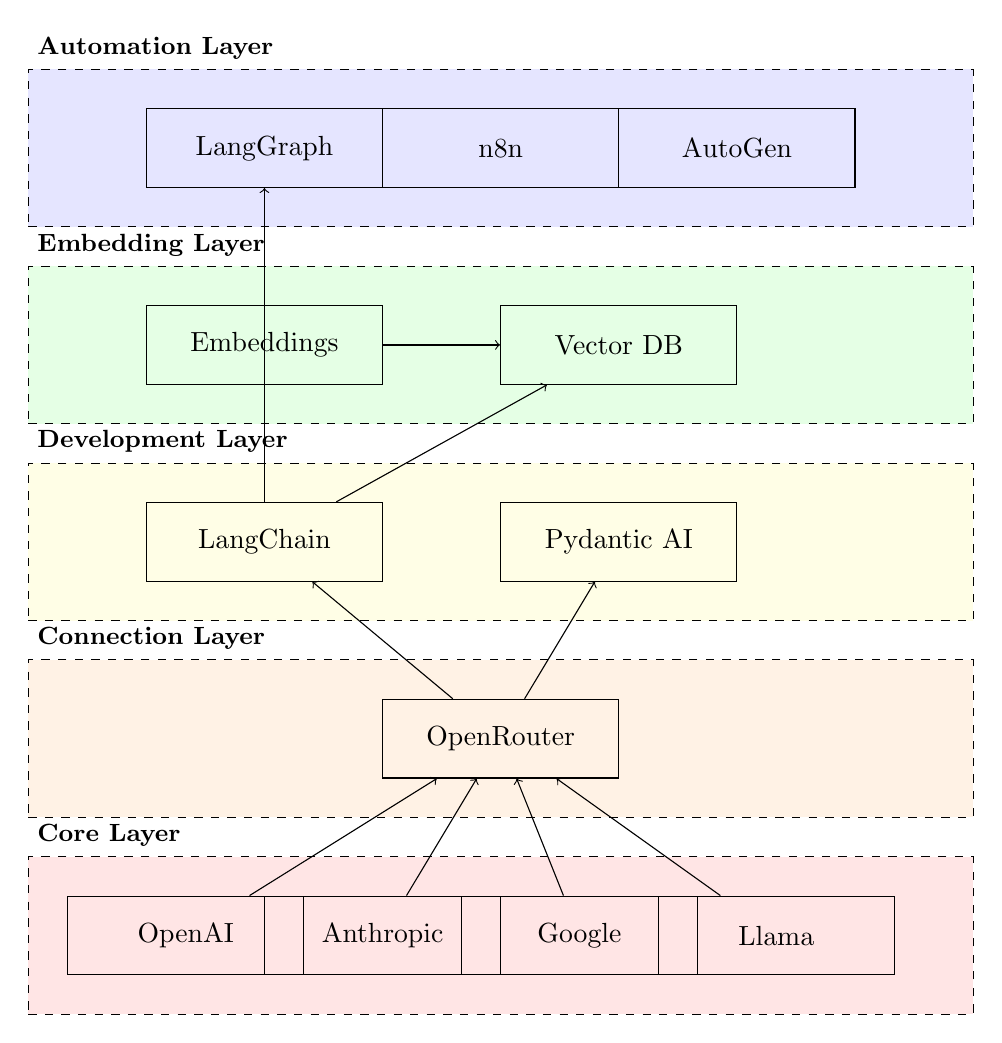
\begin{tikzpicture}[
    node distance=1.5cm,
    box/.style={rectangle, draw, minimum width=3cm, minimum height=1cm, align=center},
    layer/.style={rectangle, draw, dashed, minimum width=12cm, minimum height=2cm}
]

% Layers
\node[layer, fill=blue!10] (layer5) at (0,10) {};
\node[above right] at (layer5.north west) {\small \textbf{Automation Layer}};

\node[layer, fill=green!10] (layer4) at (0,7.5) {};
\node[above right] at (layer4.north west) {\small \textbf{Embedding Layer}};

\node[layer, fill=yellow!10] (layer3) at (0,5) {};
\node[above right] at (layer3.north west) {\small \textbf{Development Layer}};

\node[layer, fill=orange!10] (layer2) at (0,2.5) {};
\node[above right] at (layer2.north west) {\small \textbf{Connection Layer}};

\node[layer, fill=red!10] (layer1) at (0,0) {};
\node[above right] at (layer1.north west) {\small \textbf{Core Layer}};

% רכיבים
% שכבה 5
\node[box] (auto1) at (-3,10) {\textenglish{LangGraph}};
\node[box] (auto2) at (0,10) {\textenglish{n8n}};
\node[box] (auto3) at (3,10) {\textenglish{AutoGen}};

% שכבה 4
\node[box] (emb) at (-3,7.5) {\textenglish{Embeddings}};
\node[box] (vec) at (1.5,7.5) {\textenglish{Vector DB}};

% שכבה 3
\node[box] (lc) at (-3,5) {\textenglish{LangChain}};
\node[box] (py) at (1.5,5) {\textenglish{Pydantic AI}};

% שכבה 2
\node[box] (or) at (0,2.5) {\textenglish{OpenRouter}};

% שכבה 1
\node[box] (oai) at (-4,0) {\textenglish{OpenAI}};
\node[box] (ant) at (-1.5,0) {\textenglish{Anthropic}};
\node[box] (goo) at (1,0) {\textenglish{Google}};
\node[box] (lla) at (3.5,0) {\textenglish{Llama}};

% חיצים
\draw[->] (oai) -- (or);
\draw[->] (ant) -- (or);
\draw[->] (goo) -- (or);
\draw[->] (lla) -- (or);
\draw[->] (or) -- (lc);
\draw[->] (or) -- (py);
\draw[->] (lc) -- (auto1);
\draw[->] (lc) -- (vec);
\draw[->] (emb) -- (vec);

\end{tikzpicture}
\end{english}
\caption{ארכיטקטורת אקוסיסטם \en{AI} מלאה -- 5 שכבות}
\end{figure}

\subsection*{תרשים 2: גרף עמודות -- השוואת מחירים}

\begin{figure}[h]
\centering
\begin{english}
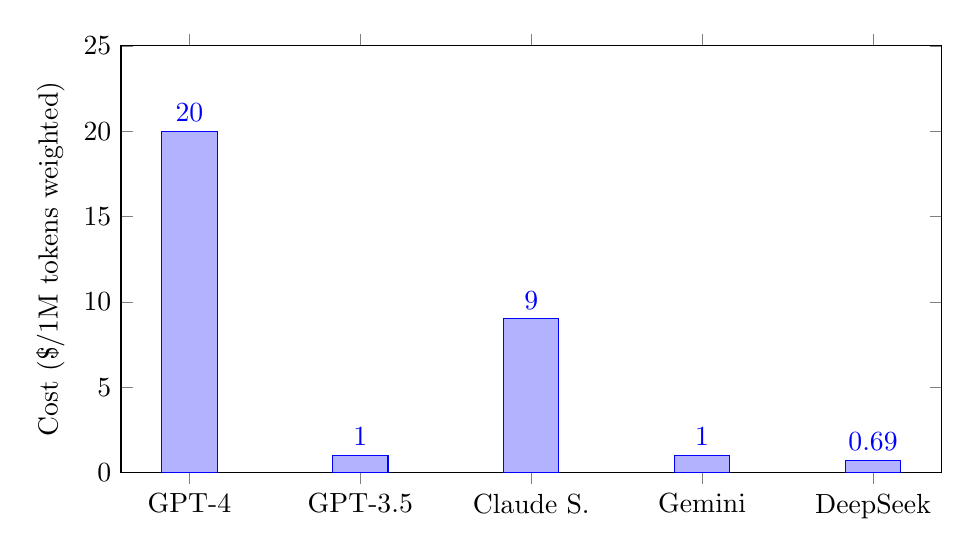
\begin{tikzpicture}
\begin{axis}[
    ybar,
    bar width=20pt,
    ylabel={Cost (\$/1M tokens weighted)},
    symbolic x coords={GPT-4, GPT-3.5, Claude S., Gemini, DeepSeek},
    xtick=data,
    ymin=0,
    ymax=25,
    nodes near coords,
    width=12cm,
    height=7cm,
]
\addplot coordinates {(GPT-4,20) (GPT-3.5,1) (Claude S.,9) (Gemini,1) (DeepSeek,0.69)};
\end{axis}
\end{tikzpicture}
\end{english}
\caption{השוואת מחירים ממוצעים בין מודלים מובילים}
\end{figure}

\subsection*{רשימת קריאה מומלצת}

\begin{itemize}
\item \textbf{LangChain Documentation} -- \en{https://python.langchain.com/}
\item \textbf{OpenRouter Models List} -- \en{https://openrouter.ai/models}
\item \textbf{Pinecone Learning Center} -- \en{https://www.pinecone.io/learn/}
\item \textbf{Anthropic Claude Documentation} -- \en{https://docs.anthropic.com/}
\item \textbf{Llama Model Card} -- \en{https://llama.meta.com/}
\end{itemize}

\end{document}
